\documentclass{beamer}
\usepackage{amsmath,amsfonts,amssymb}
\usepackage{bm}
% Theorem environments-------------------------------------------
\newtheorem{thm}{Theorem}[section]
\newtheorem{cor}[thm]{Corollary}
\newtheorem{lem}[thm]{Lemma}
\newtheorem{prop}[thm]{Proposition}
\theoremstyle{definition}
\newtheorem{defn}[thm]{Definition}
\theoremstyle{remark}
\newtheorem{rem}[thm]{Remark}
\numberwithin{equation}{section}
% simple commands---------------------------------------------
\newcommand{\abs}[1]{\left\vert#1\right\vert}
\newcommand{\set}[1]{\left\{#1\right\}}
\newcommand{\seq}[1]{\left<#1\right>}
\newcommand{\norm}[1]{\left\Vert#1\right\Vert}
%additional-------------------------------------------------------
\newtheorem{prob}{Problem}[]
%------------------------------------------------------
\begin{document}
\title{research outline}
\date{\today}
\author{Daeseok Lee}
\frame{\titlepage}
%------------------------------------------------------
\AtBeginSection[]
{
    \begin{frame}
        \frametitle{Table of Contents}
        \tableofcontents[currentsection]
    \end{frame}
}
%-----------------------------------------------------
\frame{\frametitle{table of contents}\tableofcontents}

\section{outline}
\frame{\frametitle{goals}
\begin{itemize}
\item check adaptation of traits
\item argue on "mixing-input trick" 
\item experiments for validating adaptation of behavior 
\item neural networks 
\end{itemize}

}

\section{adaptation of traits}
\frame{\frametitle{example of trait adaptation}

\large
maximum age / maximum size / nutritient accumulation rate
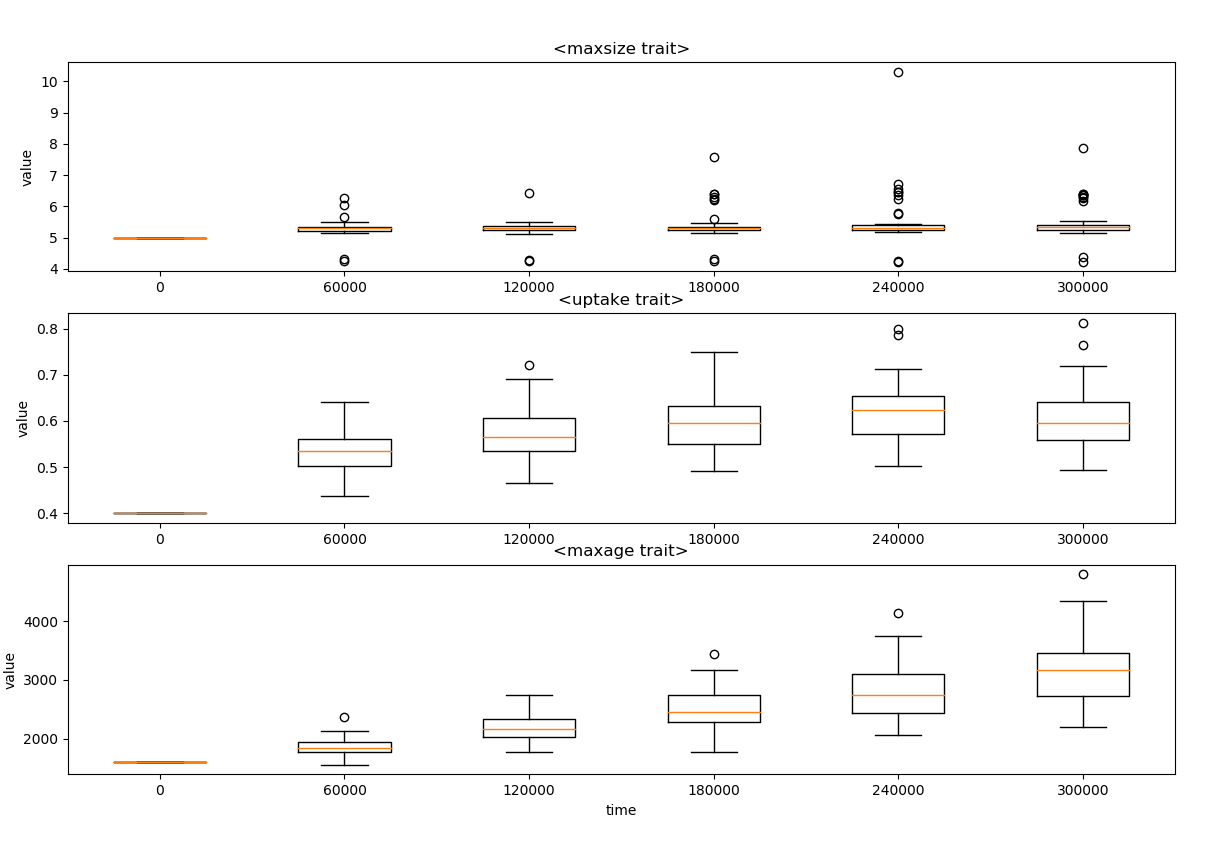
\includegraphics[width=1.0\textwidth]{/home/daese/projs/miniworld/exps/exp1/ver0.2-1/traits.png}

}

\frame{\frametitle{evidence of intelligence?!}
\includegraphics[width=1.0\textwidth]{/home/daese/projs/miniworld/exps/exp1/ver0.2-1/pc.png}
}
\frame{\frametitle{mixing input trick}
\begin{itemize}
\item randomly shuffle the input of all minions
\item elimination of input-specific behavior
\end{itemize}
\pause
\includegraphics[width=0.6\textwidth]{/home/daese/projs/miniworld/exps/exp0/ver0.2-1/pc.png}
\begin{itemize}
\item no difference??!!!
\end{itemize}
}

\frame{\frametitle{A tiny coding mistake}
\begin{itemize}
\item the mutation of color trait was implemented roughly like:
\begin{itemize}
\item $(r,g,b)=$(average of parent's)
\item $\delta r,\delta g,\delta b\sim N(0,\sigma^2)$
\item $(r',g',b')=(int(r+\delta r),int(g+\delta g),int(b+\delta b))$
\end{itemize}
\item What's wrong here??
\pause
\item "int" was implemented by python int function...
\item that returns $n$ for any $x$ such that $n\le x<n+1$
\item which has bias to the smaller integer
\end{itemize}
}
\frame{\frametitle{after fixing mistake...}
\includegraphics[width=1.0\textwidth]{/home/daese/projs/miniworld/exps/exp1/ver0.2-1/pc_after.png}
}

\section{mixing input trick}
\frame{\frametitle{scenarios}
\pause
Scenario 1
\begin{itemize}
\item The average color decreased as time passed
\item Is it due to the hunting behavior??
\end{itemize}

\pause
Scenario 2
\begin{itemize}
\item It was observed that foods are consumed more and more rapidly
\item Is it evidence of evolution of perception??
\pause
\item Not quite, it can be merely due to increased default average speed
\pause
\item Then, how do we determine whether both the speed and the intelligent caused it?
\end{itemize}
}

\begin{frame}[allowframebreaks]{logic of the trick}
\begin{itemize}
\item Let's say we observed a phenomenon P.
\item We suspect that the evolution of intelligence caused P, but we also figured out some other factors that could affected P
\item If we could eliminate the effect of "intelligence", then we might solve the problem, by seeing whether P is still observed. BUt how?
\item First attempt : just an arbitrary behavior(moment, action, etc.).$\Rightarrow$ Then not only the intelligence is affected. We have to preserved at least the "background behaviors" which has nothing to do with intelligence.
\framebreak
\item Manually figuring out some aspects of "background behaviors" and applying them to make "random behaviors" is conceivable. However, it is just an ad-hoc approach.
\item Second approach : We could supply the creatures with some "random input", which prevent them from perceive correctly and respond accordingly, thus disturbing intelligence completely. 
\item Problem : how do we generate the random input? - it should not be completely irregular. To reproduce the "background behavior", we should at least sample from the "plausible inputs"
\item Solution : randomly shuffle all the inputs!
\end{itemize} 
\end{frame}

\section{experiments}
\frame{\frametitle{outline}
\begin{itemize}
\item task-based assessments
\item harsh environment assessments\end{itemize}
}
%------------------------------------------------------
\end{document}


